% This is samplepaper.tex, a sample chapter demonstrating the
% LLNCS macro package for Springer Computer Science proceedings;
% Version 2.20 of 2017/10/04
%
\documentclass[runningheads]{llncs}
%
\usepackage{graphicx}
% Used for displaying a sample figure. If possible, figure files should
% be included in EPS format.
%
% If you use the hyperref package, please uncomment the following line
% to display URLs in blue roman font according to Springer's eBook style:
% \renewcommand\UrlFont{\color{blue}\rmfamily}

\usepackage[utf8]{inputenc}
\usepackage[caption=false]{subfig}

%% Package to include references
\usepackage[style=numeric-comp]{biblatex}
\usepackage{csquotes}
\addbibresource{Zotero.bib}

\usepackage{listingsutf8}

\usepackage{amsmath}
\usepackage{amsfonts}
\usepackage{amssymb}

\lstset{
  basicstyle=\ttfamily,
  columns=fullflexible,
  breaklines=true,
%   postbreak=\mbox{\textcolor{red}{$\hookrightarrow$}\space},
}

\begin{document}

% Allow latin letters in the code listings
\lstset{inputencoding=utf8/latin1}

%
\title{Urban Security Analysis in the City of Bogotá Using Complex Networks}
%
\titlerunning{Bogotá Urban Security Analysis}  
% abbreviated title (for running head)
% If the paper title is too long for the running head, you can set
% an abbreviated paper title here
%
\author{André Ferreira\inst{1} \and
Guillermo Rubiano\inst{2} \and
Eduardo Mojica-Nava\inst{3}\orcidID{0000-0002-3259-4013}}
%
\authorrunning{A. Ferreira et al.}
% First names are abbreviated in the running head.
% If there are more than two authors, 'et al.' is used.
%
\institute{Universidade de Lisboa - Instituto Superior Técnico, Av. Rovisco Pais 1, 1049-001 Lisbon, Portugal,\\
\email{andre.c.n.ferreira@tecnico.ulisboa.pt}
\and
Universidad Nacional de Colombia,
Cra 45, Bogotá, Colombia,\\
\email{garubianog@unal.edu.co}
\and
Universidad Nacional de Colombia,
Cra 45, Bogotá, Colombia,\\
\email{eamojican@unal.edu.co}}
%
\maketitle              % typeset the header of the contribution
%
\begin{abstract}
In an increasingly globalized and borderless world, fast access to reliable information about cities has become almost a necessity. From tourism to business trips and emigration, one should have a good knowledge about the destination to avoid problems and to ensure a good adaptation to the local region. As such, by exploring complex networks concepts and open data initiatives, this study focuses on the city of Bogotá as a model for security analysis, defined by official crime records and social strata percentages. In addition, a comparison of the previous data can be made with the location of police stations, as well as a urban traffic analysis. Finally, it's possible to do a regional quality classification and a quicker and safer route recommendation, in function of the reliable data extracted from databases, obtained from specialized institutions, with national accreditation for this work.

\keywords{Data science, big data, criminal records, network models, network visualization, open data, regional quality classification, safety analysis, social groups, urban network, urban security, urban traffic, complex systems}
\end{abstract}

%
%
%
\newpage
\section{Introduction}

The last decades have seen the reshaping of the society as information oriented. Right now, the computer is a core part of our lifes, smartphones are an extension of the human body and internet is seen as a basic need. Every document, report, event, media is digitalized, being readily accessible in a form of a PDF, a web page, a video, a database. By having the majority of the population online, constantly using and publishing more data, creation of detailed studies and impactful applications is facilitated. Beyond innovations such as online shared knowledge and social networks, this abundance of information allows the rise of data science, bringing with it the possibility to do profound analysis of the complex systems that govern the functioning of social, biological and mechanical environments. A set of complex systems that have a considerable relevance is that of urban analysis. As cities continue to grow and absorb an increasingly large chunk of the world's population, the interest for studies regarding each city goes up. As such, nowadays it's possible to find analysis regarding the touristic value and landmarks, the average health quality, the university rankings, the fastest routes to travel through the city, the economic and social status, among others. However, it's not straightforward to find objective information concerning urban security. Although there's an unprecedented quantity of data from all around the world available online, when searching for factual safety clues about a city, there's usually only personal opinions available, that don't allow for an unbiased and detailed representation of the real system. There are academic papers that attempt to tackle this situation, as will be addressed in the related work section. Having said that, these tend to lack a clear visualization of a complete safety status of a metropolis, at a neighborhood level.

In this paper, an urban safety and traffic analysis of the city of Bogotá is presented, showing an intuitive and detailed representation of the obtained data. Bogotá is the capital of Colombia, has an estimated 8 million inhabitants and, to our best knowledge, never had a urban security report published online. As such, this represented an interesting challenge, considering the size of the city, and consequently the amount of data needed, as well as an opportunity to do an unprecedented security study, in a city that has a violent past. To address this project, we need to start by figuring out how to get a data structure that could allow us to have a geographically accurate representation of the city. Considering the generic layout of cities as streets that have intersection points, it becomes clear that a network graph, which is also used as the data format in other studies \cite{geoff_osmnx:_2017} \cite{spadon_complex_2016} and in services such as Google Maps, is an adequate solution. Then, we need to be able to actually create a network variable that contains the streets structure of Bogotá, as well as coordinates. After this is done, reliable and relevant data must be fetched in order to be able to do an objective safety and traffic analysis. When the graph and the data are obtained, it's a matter of carefully weighting the variables to obtain safety and traffic values for each node and edge, visualize this information in intuitive ways and derive conclusions from it.


\section{Related Work}

To this date, a series of studies related to urban security and traffic have been published. This is due to the increasing relevance of these two problems. With the growth of cities into big metropolis, bringing socioeconomic inequalities and a greater number of vehicles that move through the streets, there's an increase in criminality and congestion. By modeling cities as complex systems through graph theory, researchers have been able to, in some way, address these issues.

Ciccato and Uittenbogaard \cite{ceccato_space-time_2012} worked on an interesting analysis on clusters of crime in Stockholm, Sweden. The study allowed a view of the regions of the Scandinavian city with more criminal activity, divided on violence and property crimes, and did a detailed time study, comparing day and night as well as winter and summer, in terms of criminal occurrences. In spite of this, there are some drawbacks to this paper. First of all, it relies on one single information from one single source, that is the crime records of Stockholm between 2006 and 2009. This means that there are no socioeconomic aspects considered, no traffic analysis and no data regarding police stations locations. Furthermore, by using the GIS framework instead of a complex networks approach, there's only a simplified visualization of the city's neighborhoods, with no possibility to view at the street level, making it difficult to extend to further research using the same data structure and preventing the functionality of calculating the best paths around the city, through use of distance and the safety knowledge gathered.


The work of Spadon et al. \cite{spadon_complex_2016} analyzes criminal communities of San Francisco, using a complex networks representation of the city, obtained directly from Open Street Maps \cite{noauthor_open_nodate} APIs, with no corrections to the graph. Based on spatial mappings of urban crimes, they proceed with an identification of criminal communities and classification according to different types of crimes. One of the main conclusions of the paper is that different crime types share common spaces, characterizing areas that lack strategies for crime prevention. This validates our simplification of considering crime as a whole, without differentiating into different types. Although there are some important methods used in this work which are similar to ours, such as using a complex networks representation and getting spatial criminal activity data, there are some flaws which we try to address. For instances, the safety analysis focuses on the most criminal intensive region of San Francisco, instead of analyzing the whole city with unsafety scores. The security information only contemplates a criminal activity dataset, without adding data such as socioeconomic aspects, which can have an impact on a neighborhood's safety. There is no use of police stations locations in the safety analysis and they didn't take advantage of the graph structure to integrate a best path routing, in terms of both travel time and safety. A traffic analysis is completely absent.

In a 2016 paper by Sol{\'e}-Ribalta et al. \cite{albert_model_2016}, it's presented a model based on the emergence of critical congestion phenomena, evidenced in complex networks, which allows to analytically predict the most influential points of vehicular congestion in the urban environment, based on real traffic information. Although it's a detailed approach to traffic analysis, it doesn't cover the topic of urban safety.

Geoff Boeing \cite{geoff_osmnx:_2017} introduced a novel complex networks tool for urban analysis, introducing the Python package OSMnx. As a new open source tool for the investigation of road networks, where one can download, analyze and build networks, a case study is discussed concerning the city of Portland, Oregon. The study consists in comparing three neighborhoods, from both metric and topological perspectives, using OSMnx. Network features such as density, connectedness, centrality, and resilience are used. In 2018, there was a publication further testing the limits of OSMnx, by doing an extensive urban morphology analysis to 27000 US cities \cite{boeing_multi-scale_2018}. It's clear that both papers don't address the topics of security and traffic. However, this tool is of great help for our research, considering that by obtaining a directed graph that represents the road fabric of the city of Bogotá, it's possible to add any type of information that facilitates the understanding and visualization of georeferenced data.

In fact, our work differs from the aforementioned because it includes specific elements, highlighted as useful from previous research, in order to unify them and integrate more variables to the problems of criminality and congestion, as is the case of the relationship of security with police checkpoints. An intuitive visualization of the whole city's street network, classified by security and by traffic, which wasn't found in any previous study, is made available. In addition, we implement a route optimization where the distance traveled is shorter and, at the same time, has less traffic jams and safer with respect to other possible paths.


\section{Methodology}

Considering the nature of the study as being one of data science and network science, all of the implementation and analysis segments revolved around the python programming language. With a strong community, releasing packages such as numpy, for numeric operations, pandas, for data analysis, networkx, for manipulating complex networks, among many others, Python has increasingly been establishing itself as the main tool for data scientists and, with the field's growth, the applicability in machine learning and its flexibility for other domains, have made it one of the fastest growing programming languages \cite{robinson_why_2017}. Furthermore, considering its readability and simplicity, it allows for a more readable code, that makes it easier for anyone to review and reuse the code, as well as allowing to do a faster code development, without having memory leaks or other possible coding issues that can delay the study. Having in mind this decision of using Python as the core tool in the methodology of the study, there are 5 main steps to get the desired data analysis:

\begin{enumerate}
	\item City graph
    
    \item Security data
    
    \item Traffic data
    
    \item Police stations locations
    
    \item Edge weight calculation
\end{enumerate}

In the following pages, each of these steps are explained in further detail.

\subsection{City Graph}

A graph, or a network, has two main components: edges and nodes. Nodes represent possible points of interest, data points that can have practically any positive finite dimensionality. Edges represent connections between nodes, which can either be bidirectional or unidirectional, have the option of not existing at all between two given nodes and can have an attributed weight, which can be calculated as a function of certain dimensions of the end nodes. 
When thinking about a city, wherever it may be in the world, there are two things that are always present: streets and their inevitable intersections. Intersections can be seen as the nodes of a city, representing points of the urban landscape, where, besides geographical coordinates, dimensions can be added to represent the levels of insecurity and traffic congestion of the surroundings. The streets themselves can be seen as the edges of a city graph, which connect pairs of intersections, if there is a road between them, is either bidirectional or unidirectional, depending on whether the road is two-ways or one-way, and has a weight, which can be calculated based on a combination of the distance between the intersections, the security and traffic characteristics of the nodes' neighborhoods. All of this makes it clear that, using the streets connections, it's possible to have a network representation of a city. But now there's the problem of how to get the geographical information of a city's road map, namely of Bogotá, and how to set the intersections and their respective road connections. To handle this task, the OSMnx \cite{geoff_osmnx:_2017} Python package is the right tool.

OSMnx \cite{geoff_osmnx:_2017} is a Python package developed by Geoff Boeing, a postdoctoral Researcher at University of California, Berkeley. With it, it's possible to download spatial geometries and construct, project, visualize, and analyze street networks from OpenStreetMap’s APIs \cite{noauthor_open_nodate}. OSMnx \cite{geoff_osmnx:_2017} improves the graphs of OpenStreetMap by only keeping the nodes which represent true street intersections and concatenates the edges that connected the intermediate false nodes into a single edge between two intersection nodes. Besides this network simplification, by being built on top of other packages such as geopandas, networkx, and matplotlib, OSMnx \cite{geoff_osmnx:_2017} gives access to powerful graph manipulation, graph visualization tools and path routing techniques, while additionally implementing some automatic graph analysis such as betweenness centrality, network circuity, streets per node proportions, average edge length in meters, among others.

Although OSMnx \cite{geoff_osmnx:_2017} allows fetching the urban network with the right political borders just by using the city's name, this feature only works for specific cities. Since it doesn't work for Bogotá, one needs to indicate a center point of the city in geographical coordinates and select a range in meters that will select the furthest away a node can be from the center. This way, it's not possible to get the right city map, but rather a graph that contains some nodes from nearby towns. By selecting a point in the center of Bogotá and a range of 20 km, the graph from figure \ref{fig:FirstBogGraph} is constructed.

\begin{figure}[!h]
  \centering
  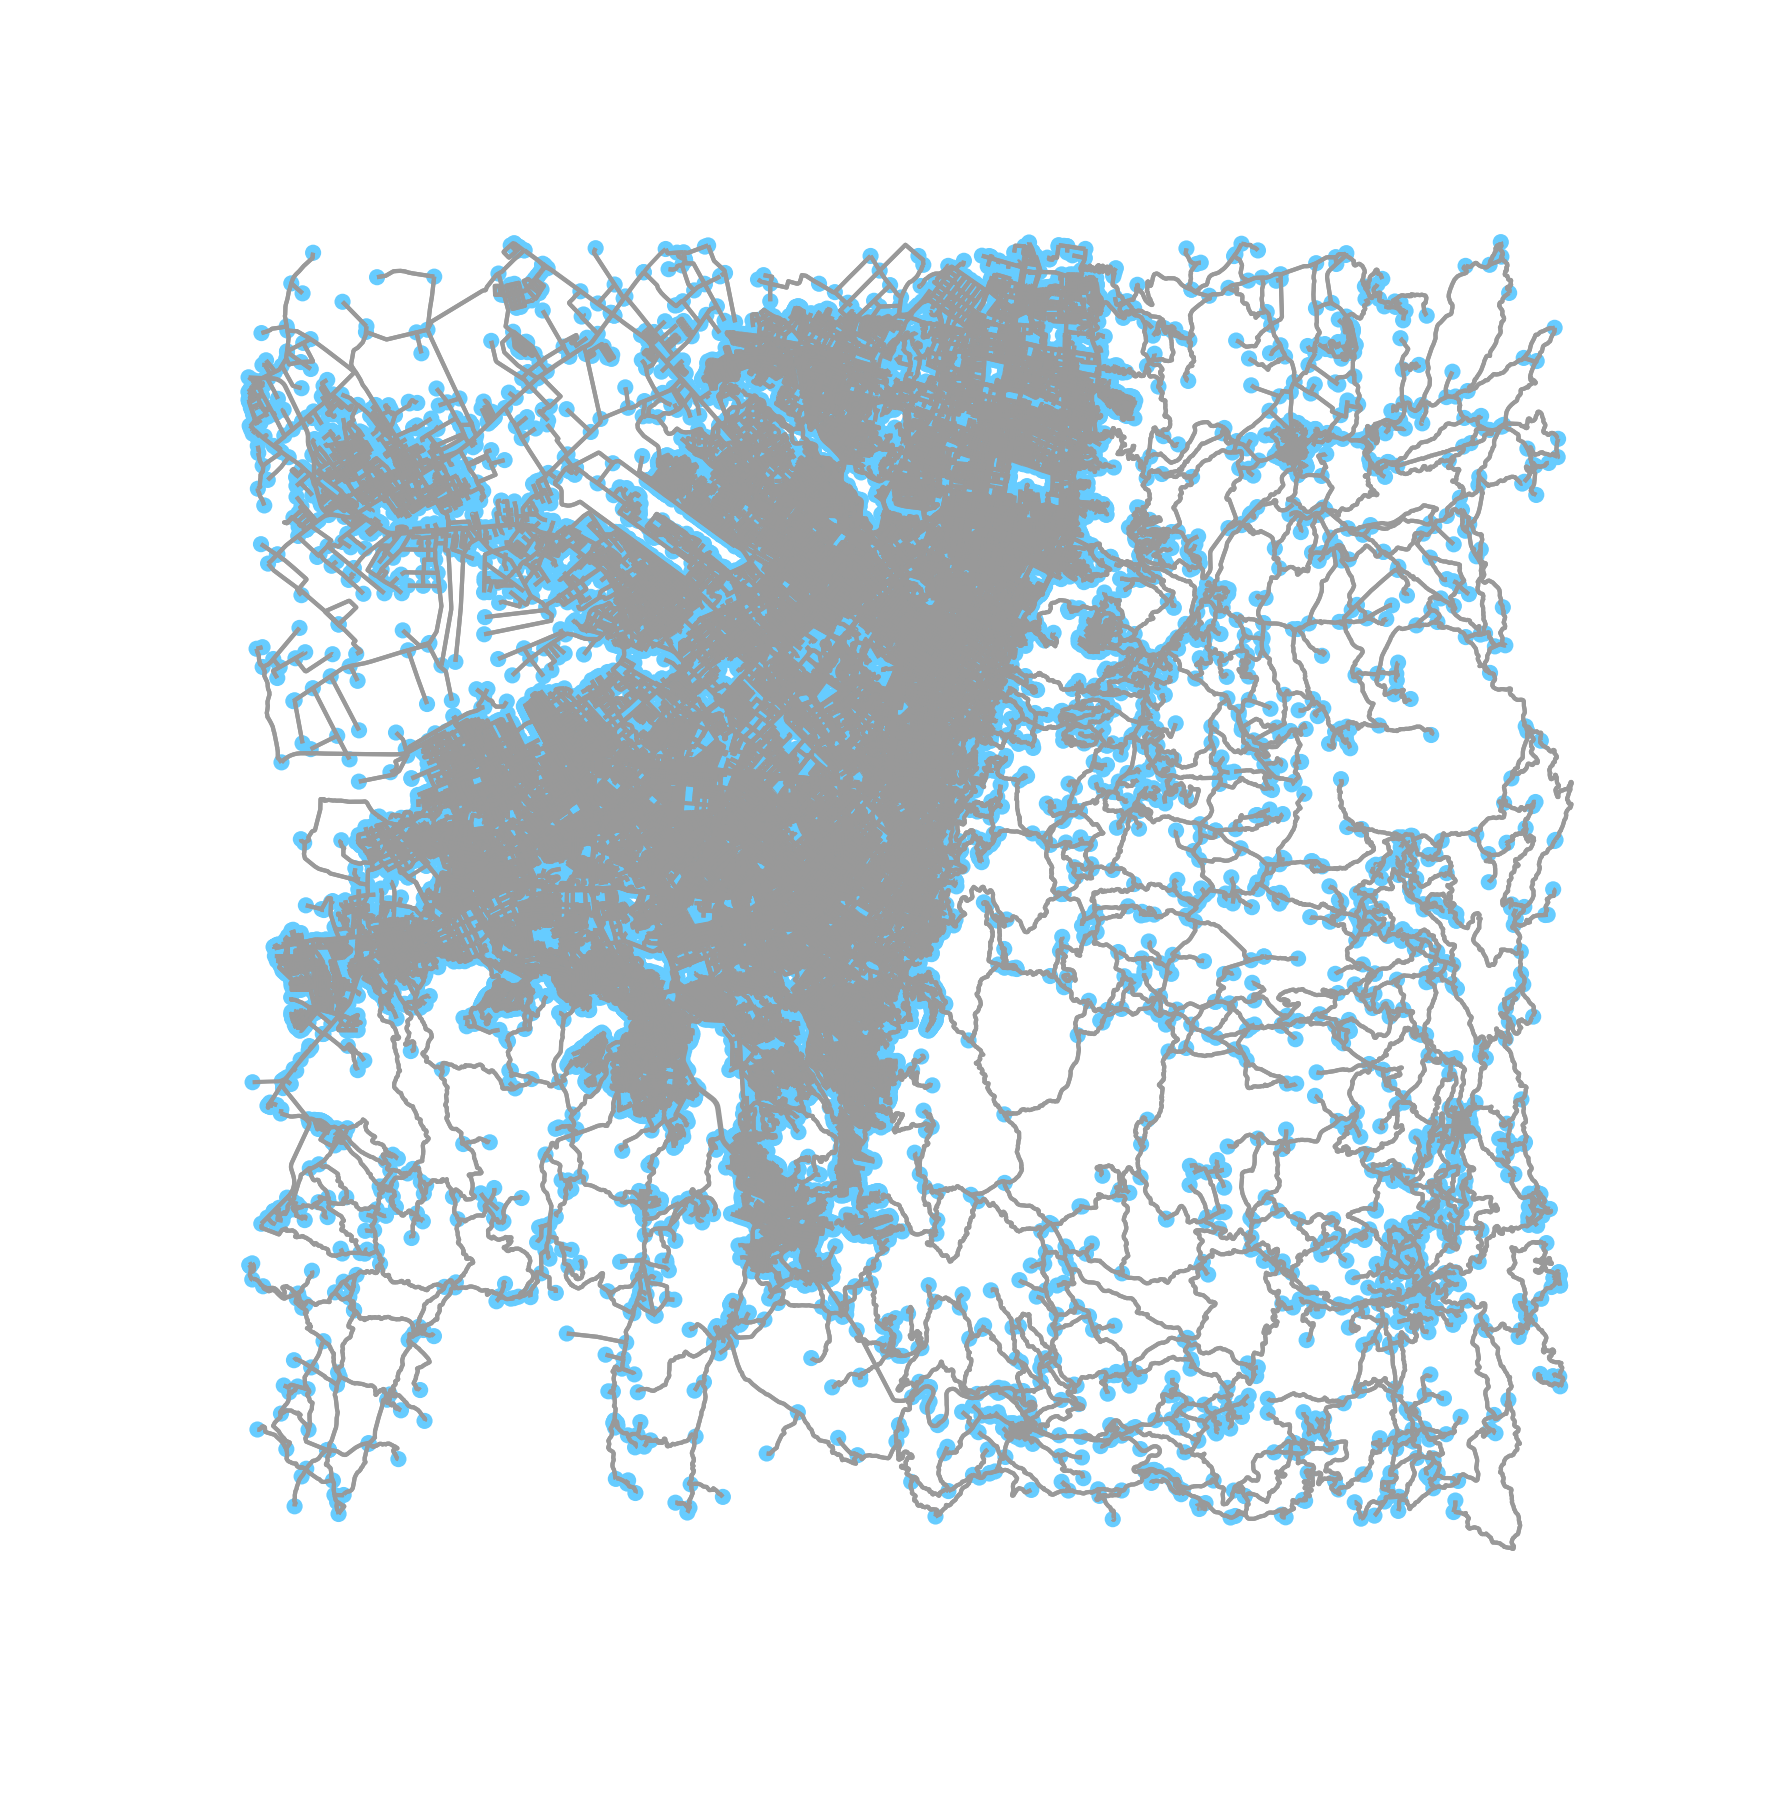
\includegraphics[width=.7\textwidth]{Images/GrafoBogota.eps}
  \caption{Network graph representing the city of Bogotá, Colombia, as well as its surroundings, obtained with OSMnx.}
  \label{fig:FirstBogGraph}
\end{figure}


\newpage
\subsection{Security Data}

One of the most relevant sources of data that an urban security study can have is that of criminal activity logs. By having a factual account of all the criminal occurrences that happened in a city during a given interval of years, with a geographical location of the infringement and possibly the type of crime, it enables the making of studies that can objectively classify a city's regions according to a unsafety score. This hypothesis is widely accepted, as it can be seen being applied by various studies \cite{ceccato_space-time_2012} \cite{spadon_complex_2016}. However, in order for this to work flawlessly, there would need to be (i) enough data, which means having a long time interval of crime records, (ii) a time span in which the criminal panorama remains sufficiently stable, as one should have data that corresponds as much as it can to the current situation, (iii) truthful data, as having crimes registered in the wrong location or even false crimes can mess up the analysis, and (iv) no missing data, as absolutely all criminal events that occurred during the dataset's time span must be registered in order for the data analysis to be perfectly representative of the real world. Considering that these requirements aren't easy to pass, that it's practically impossible to confirm a dataset's complete verification of the requirements and that this paper analysis the city of Bogotá, which has around 8 million inhabitants, making it harder to register every single crime in a dataset and validate it, we consider that there should be a better way to get the safety information.

Many studies show that there's a causal effect of poverty on crime, violence and social unrest \cite{iyer_poverty_2014} \cite{lagi_food_2011}. As such, by having some dataset that can detail the proportion of people living in poverty conditions in each city region, it would be valuable information to determine the safety of a given region. As Bogotá has an official social stratum register, calculated through the values of the residential buildings and their corresponding terrain, it's straightforward to use a dataset from SISCRED \cite{secretaria_de_cultura_recreacion_y_deporte_siscred_nodate}, the municipality's information system, containing the number of inhabitants in each neighborhood, as well as their social stratum. In this case, for each neighborhood, we're counting on the number people from the two lowest strata and the ones without stratum, as it usually happens in Bogotá that these correspond to citizens with low income living in illegal conditions. Afterwards, we divide that number by the total amount of inhabitants of the neighborhood, resulting in the equation $Pvr_{p_i} = \frac{P_{ns_i} + P_{s_{1_i}} + P_{s_{2_i}}}{P_i}$, where $Pvr_{d_i}$ corresponds to the poverty proportion of the population, $P_{ns_i}$ is the number of inhabitants without stratum, $P_{s_{1_i}}$ is the number of inhabitants in stratum 1, which is the lowest in Colombian standards, $P_{s_{2_i}}$ is the number of inhabitants in stratum 2, which is the second lowest in Colombian standards, and $P_i$ is the total amount of inhabitants, all referring to the the neighborhood of node $i$.

Similarly, regarding the criminal activity data, we gathered a dataset from Open Data Bogotá \cite{camara_de_comercio_de_bogota_open_nodate}, an open data initiative from the city's governance, containing criminal activity logs from 1985 until 2015. Considering that the data should be representative of the present, we filter the file to crimes committed between 2010 and 2015, which gets us 59225 criminal activities, such as assaults, bank robberies, shop robberies, violence and homicides, registered during those years. Unfortunately, the location associated to each crime is only it's locality, which is a subdivision of the city of Bogotá containing multiple neighborhoods. In spite of this, it still is useful information to determine the security level of each part of the city. As such, the way to proceed is to get the number of crimes registered in a locality, $Crm_i$, and divide it by the number of inhabitants of that locality, $P_i$, resulting in a criminal density, $C_{d_i}$, independent of a region's population dimension. This is equivalent to using the equation $C_{d_i} = \frac{Crm_i}{P_i}$ to determine the criminal density for each node of the graph.

Knowing that we're using a graph structure to represent the city, having the streets intersections as nodes of the graph, it's reasonable to add a new dimension to each node for a unsafety score, consisting of a weighted sum between the criminal density and the poverty proportion of the population in that node's neighborhood. As such, it's just the matter of extracting the data from each dataset's xlsx file using the pandas Python package, setting the weight parameters, $k_{c}$ and $k_{p}$, and proceeding with the calculations to pin down each node's unsafety score, $Unsafety\_score_i$. Considering that the mean value of the criminal density is about 10 times lower than that of the poverty proportion, $k_{c}$ should be bigger than $k_{p}$, in order to compensate for the difference of average values. This way, the influence that each unsafety factor has is more balanced.

$$Unsafety\_score_i = k_{c} C_{d_i} + k_{p} Pvr_{d_i}$$


\subsection{Traffic Data}

In essence, road traffic congestions are a result of having a lot of people riding cars, trucks or motorcycles, on the same pathway, at the same time. As such, the main causes for this problem can be attributed to the number of people living or commuting in a given area and to the available options for traveling between different points in the city. This last part could be addressed by evaluating characteristics such as connectivity and centrality of each node of the obtained graph, considering that a street network with a corresponding graph that has many connections should reduce traffic congestions, due to having a lot of available routes, while a high betweenness centrality value in a small set of nodes should increase traffic congestions, due to the existence of a small set of points through which a lot of people must travel through. However, we aren't going to analyze this aspect of traffic, although we'll consider it for future work. Instead, we focus on the problem related to the number of people or, more precisely, the population density. This has been shown to have a proportional relation with daily traveling delay in several studies \cite{levinson_network_2012} \cite{louf_how_2014}. Having this in consideration, a Bogotá mobility dataset from DANE \cite{gobierno_de_colombia_dane_nodate}, the national statistics institute of Colombia, is used, filtering the data to get just the population density. The dataset gives a population density value of number of inhabitants per square kilometer, for each locality. As a locality is a group of multiple neighborhoods, this doesn't allow a very detailed analysis of traffic, but does enable a broad view of possible congestion issues in certain regions of the city. Having this in consideration, the traffic score that is added to each node, $Traffic\_score_i$, is the population density of the node's locality, $P_{d_i}$, fetched directly from DANE's dataset \cite{gobierno_de_colombia_dane_nodate}.

$$Traffic\_score_i = P_{d_i}$$

In summary, each non police station node of the graph has the following values:

$$n_i = (Latitude, Longitude, Address, Unsafety\_score, Traffic\_score)_i$$

Where $Latitude$ and $Longitude$ are obtained from OSMnx \cite{geoff_osmnx:_2017}, $Unsafety\_score$ and $Traffic\_score$ are calculated as shown before, and the $Address$ is the neighborhood with a central point that has the shortest distance to the node. Each neighborhood's central coordinates are found through the Google Maps geocoder, implemented in the geopy \cite{noauthor_geopy_nodate} Python package.

\subsection{Police Stations Locations}

% Escribe acá Guillermo:
Counting on the information of the police stations in the city, together with the crime and congestion data, one can test to see if there are possible existing correlations between the variables, verifying in what way each characteristic can be influenced by the other. For example, assuming that police stations all have comparable performance quality, we expect that, in places where the presence of police stations is higher, crime rates are lower than in locations with fewer police stations.

For information on the location of police stations in the city of Bogotá, we first experimented with Google Maps Places API, which allows to perform queries in an area defined with central geographic coordinates and a radius. As such, by performing the query for police stations through the API in Python, we should receive the names and coordinates of all the police stations. However, the amount of information returned by the medium of this service was not considerable or relevant in relation to the number of police checkpoints, as the resulting list had a maximum size of 80, which doesn't actually correspond to real life, considering the size of the city of Bogotá. For this reason, starting from the same source, Google Maps, a manual search for each of the places of interest is performed. We select these manually and store in a Google account, in the favorite places section, to have this information available when required. Finally, after downloading the coordinates and names of the police stations in a KML file, it's implemented a reading method in Python to look in the KML file for each search result and add it to our graph as police nodes. This is what makes it possible to locate the police stations and assign an attribute or specific name for the identification of the objects in the street network. As such, each node corresponding to a police station has 4 dimensions:

$$n_i = (Latitude, Longitude, Name, Type)_i$$

The $Type$ dimension serves to clarify that the node is a police station.

\subsection{Edge Weight Calculation}

As it would be expected in a street network, OSMnx \cite{geoff_osmnx:_2017} utilizes short path optimization methods from networkx to calculate the route between two nodes that has the shortest distance, allowing to plot this path on the graph afterwards. The way this works is, by starting from the initial node, seeing which set of edges, that lead to the destination node, have weights such that there summation constitutes a minimum value. This means that the main parameter for calculating the best route is the edges' weights, which is just one value of one dimension of the edges in OSMnx. In essence, one can modify the edges' weights in order to change the relevant factors for optimal routing. In our point of view, there are two principal attributes that any person wants to have maximized on a route, which are fast and safe. The fast attribute is partially solved, as the default edge weight represents the distance between two intersections. However, considering the influence of traffic in transit time, the distance isn't enough to determine the fastness of a route. As such, the traffic data that was added to every node should be considered. Meanwhile, for the safe attribute, we already have a unsafety score in every node of the network. Taking all of this into account, the next logical step is to recalculate each edge's weight as a weighted sum of the distance, traffic score and unsafety score. 

$$w_{ij} = k_d dist_{ij} + k_s saf_{ij} + k_t traf_{ij}$$

$w$ represents the weight of the edge that connects nodes $i$ and $j$, in which $dist_{ij}$, $saf_{ij}$ and $traf_{ij}$ represent the distance, safety and traffic attribute of the edge, respectively, while $k_d$, $k_s$ and $k_t$ represent each dimension's weight on the calculation. The $k$ weights are parameters that are manually tuned, according to the priority that the current user gives to the distance of the route, the safety and the traffic conditions of the neighborhoods. The remaining variables are determined using the following expressions:

$$dist_{ij} = \text{Obtained from Open Street Maps}$$

$$saf_{ij} = \frac{Unsafety\_score_{i} + Unsafety\_score_{j}}{2}$$ 

$$traf_{ij} = \frac{Traffic\_score_{i} + Traffic\_score_{j}}{2}$$


\section{Results}

In this section, the main results are presented and discussed, separating the analysis in the four topics addressed by this study.

\subsection{Network and Traffic Information}

As was discussed before, OSMnx \cite{geoff_osmnx:_2017} allows for a detailed urban morphology analysis. Using this tool, it's possible to get interesting information regarding a city viewed as a complex network. For instances, with respect to the graph obtained for the city of Bogotá, we get 89543 nodes, which represent street intersections, 236881 edges, which are every directed connection between nodes, and 133394 street segments, which are less than the edges due to considering a street in both one-way or two-way paths. Considering also the attributes regarding average street length, average streets per node and average circuity, which relates to the curvilinearity of the streets by measuring the ratio of edge lengths to the great-circle distances between the connected nodes, one can compare the complex network of Bogotá with that of some of the biggest cities in the US, using the data collected by Geoff Boeing with OSMnx \cite{boeing_multi-scale_2018}. As a way of doing a traffic analysis, we also added information regarding population density, from census data available on Wikipedia, and also the impact of traffic congestion, from the 2017 INRIX Global Traffic Scorecard \cite{noauthor_inrix_2017}, which is a study that gives a city ranking, in which a lower number corresponds to a worse congestion problem, based on an evaluation of urban travel, traffic health and vibrancy.

\begin{table}
  \caption{Complex street networks comparison between Bogotá and some of the biggest US cities, in terms of population. Presented in descending order by population density.}\label{tab1}
  \begin{center}
  \begin{tabular}{|l|l|l|l|l|l|}
    \hline
    City & Population Density & Avg. Street & Avg. Streets & Avg. & 2017 INRIX Traffic \\
     & [People / km\textsuperscript{2}] & Length [m] & Per Node & Circuity & Scorecard Rank \\
    \hline
    New York & 11000 & 148 & 2.86 & 1.06 & 3 \\
    Boston & 5368 & 154 & 2.71 & 1.09 & 14 \\
    Bogotá & 5092 & 85 & 2.97 & 1.08 & 6 \\
    Miami & 4866 & 149 & 2.89 & 1.10 & 10 \\
    Chicago & 4594 & 163 & 2.92 & 1.07 & 17 \\
    Philadelphia & 4512 & 159 & 2.87 & 1.08 & 52 \\
    Los Angeles & 3275 & 151 & 2.82 & 1.06 & 1 \\
    Houston & 1414 & 145 & 2.83 & 1.08 & 26 \\
    \hline
  \end{tabular}
  \end{center}
\end{table}

Looking at table \ref{tab1}, something that is immediately noticeable is the significant difference of the average street length of Bogotá, compared to the other cities. This can be due to an alternative street pattern, as Bogotá is the only non-US city on the table, but also because the graph that was obtained for Bogotá, as was explained before, doesn't have the political borders of the city, ending up englobing some small neighboring towns like Madrid and Choachí, which can have shorter roads. Another interesting observation is that, as foreseen by other studies \cite{levinson_network_2012} \cite{louf_how_2014}, there does seem to be a relation between population density and traffic congestions, as in general the most densely populated cities have a higher INRIX rankings than those less densely populated. However, there are exceptions such as Boston, Los Angeles and Houston, as they all have a ranking that is higher than a previous city on the list. Besides other factors that aren't displayed on the table, such as the fact that Bogotá doesn't have a subway transport system, Los Angeles and Houston have a lower average street length than Chicago and Philadelphia, overturning the population density differences, and both Bogotá and Miami also have a lower average street length than Boston, making them higher ranked in the traffic scorecard, despite being slightly less densely populated. There also seems to be a negative effect of low circuity on traffic, as some of the worst ranked cities of the list also have the lowest average circuity, such as the case of Los Angeles which is on a high position of the rank with New York, having a big difference in population density but sharing the lowest circuity of the cities in the table. This is probably due to the fact that a lower circuity means a more grid like street pattern, presenting more intersections, stops and traffic lights than a curvier, higher circuity street geometry.

\begin{figure}[h]
	\centering
	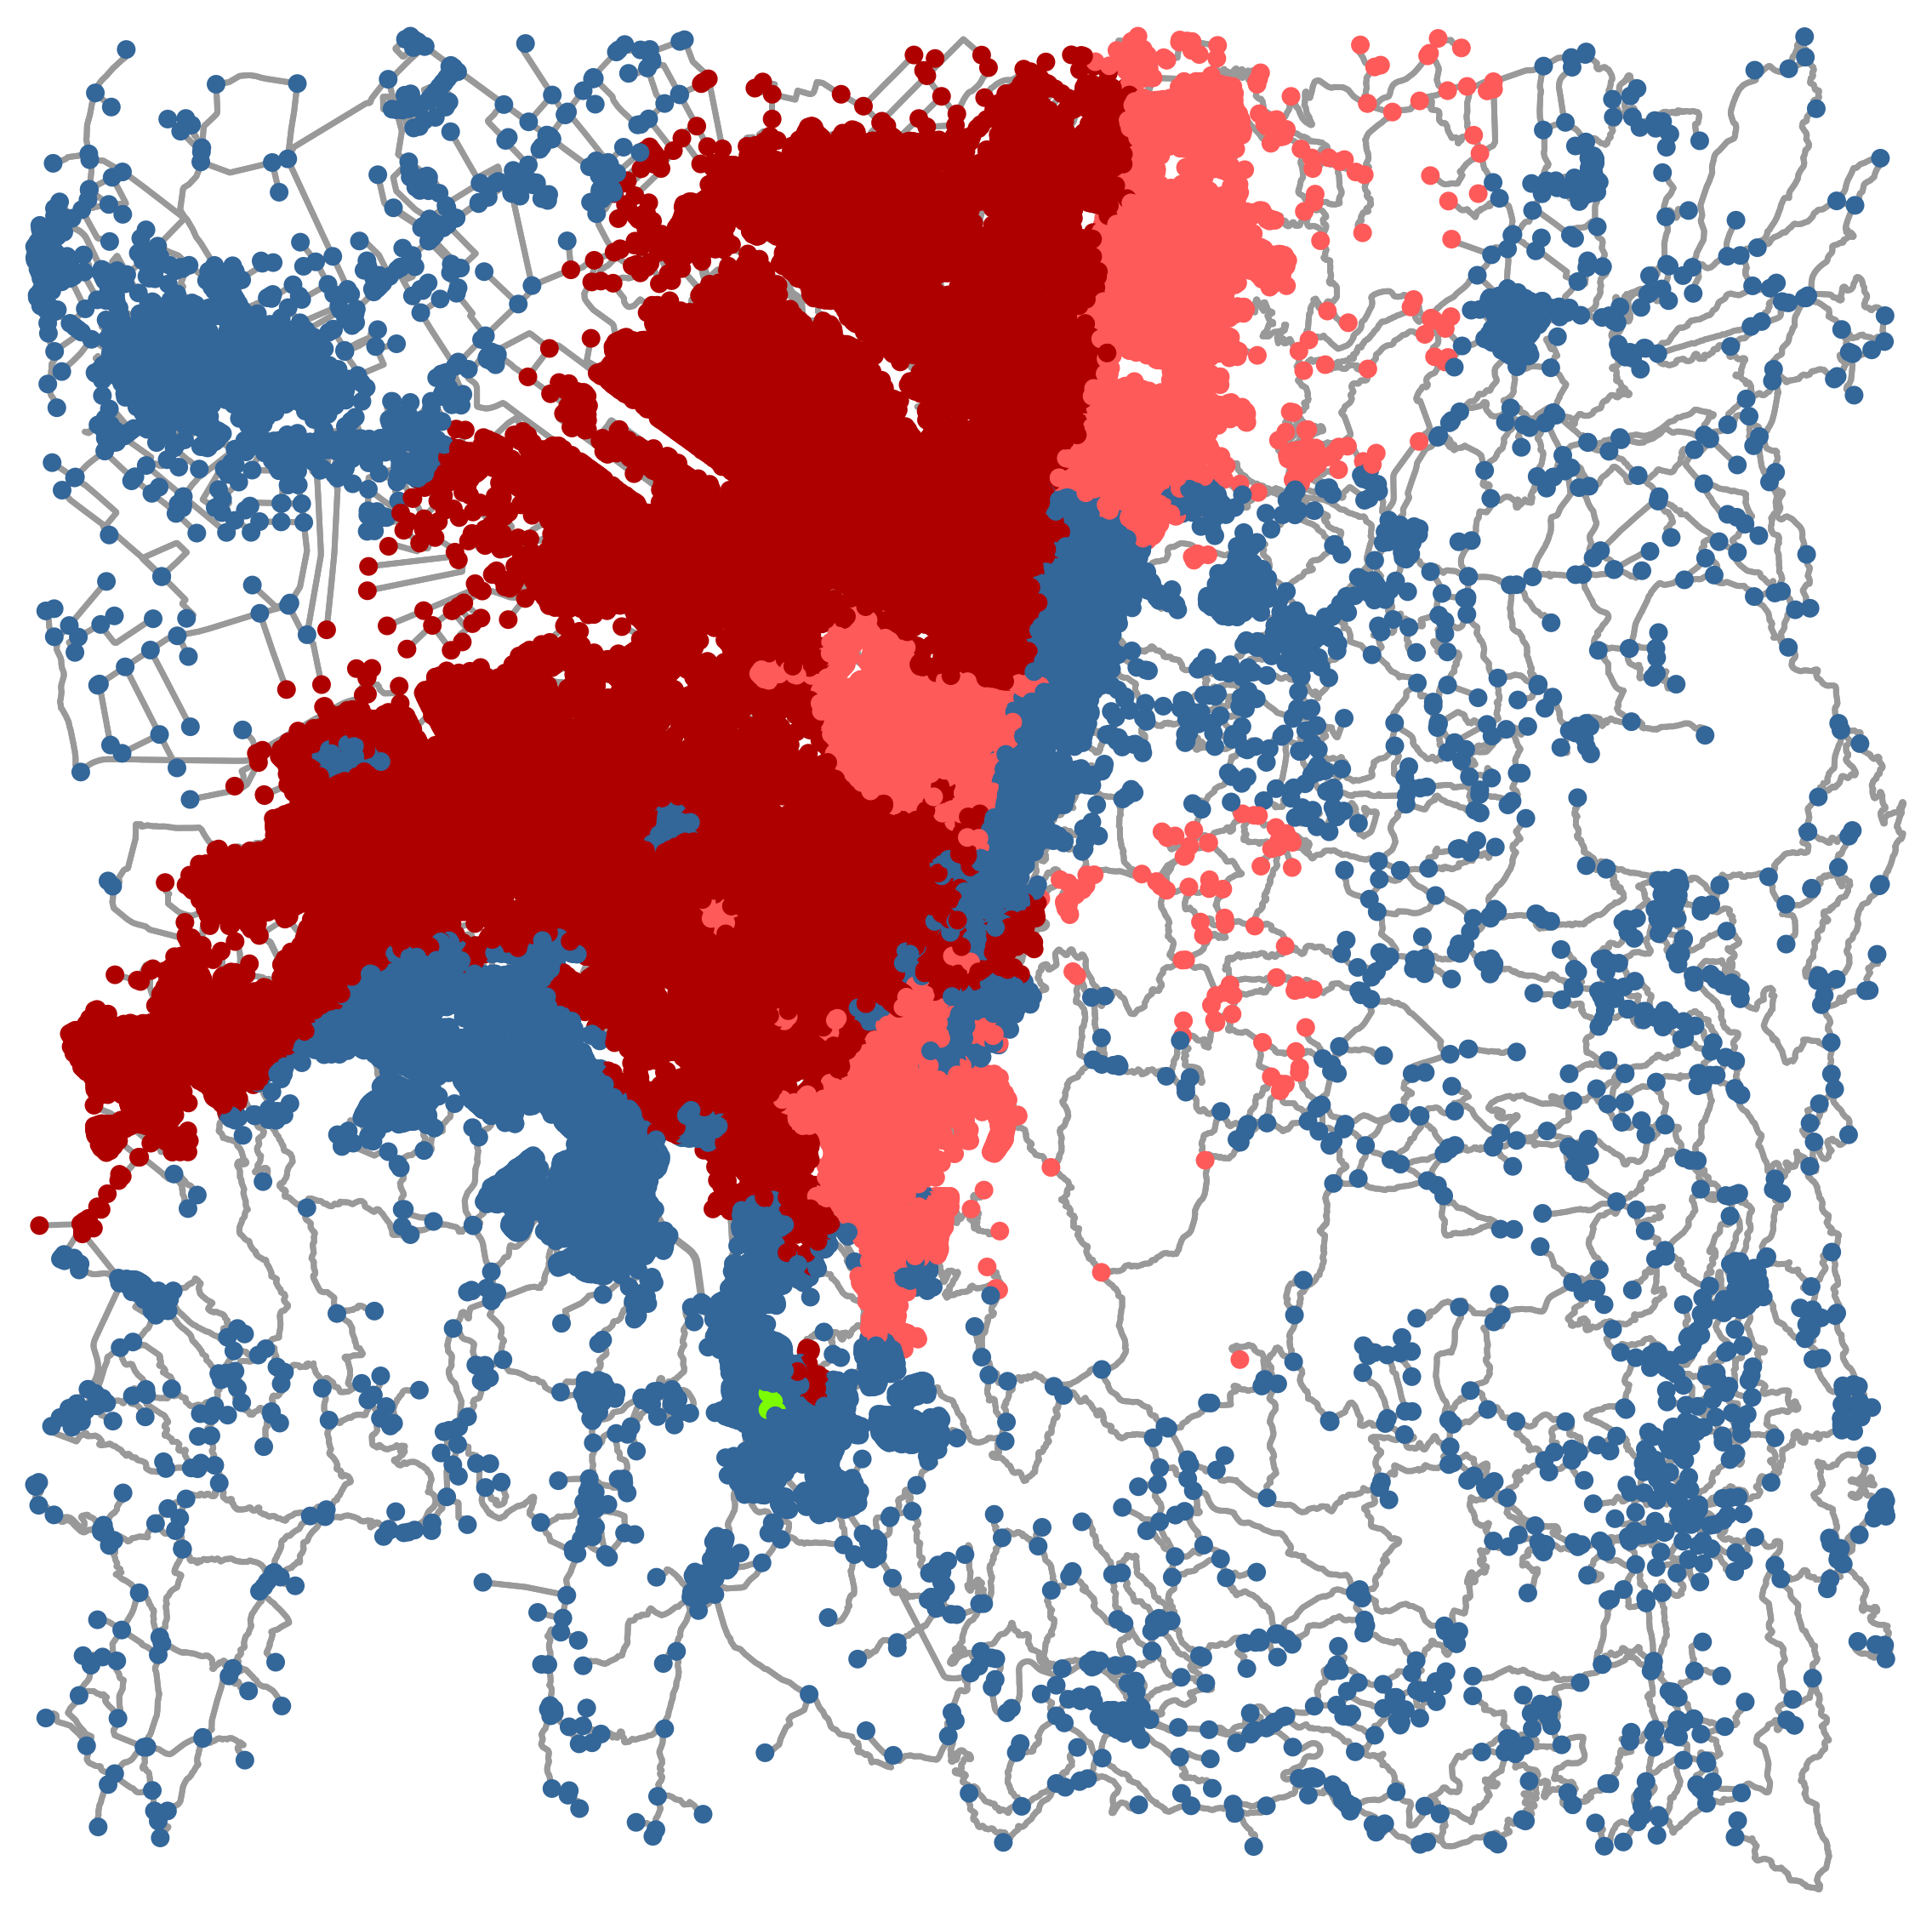
\includegraphics[width=0.5\textwidth]{Images/GrafoBogotaTrafico}
	\caption{Traffic data visualization on the graph of the city of Bogotá, with dark red colors representing higher congestion risk.}
    \label{fig:Traffic}
\end{figure}

Figure \ref{fig:Traffic} is the result of visualizing the graph nodes' traffic score, using as thresholds a population density higher than 6000 people / km\textsuperscript{2} for the light red color and higher than 11000 for the darker red color, with all the remaining nodes having a blue color. It might seem to be a contradiction that there's such a big segment of the city with a population density higher than 11000 people / km\textsuperscript{2} and having the census saying that the city has an average population density of only 5092 people / km\textsuperscript{2}. However, this is due to the highly changeable landscape of the Colombian capital, having modern skyscrapers but also lower densed neighborhoods, such as Chapinero, and a big rural area, with a relatively small number of inhabitants. Nevertheless, the big concentration of people in central and northern areas of Bogotá, comparable in population density to New York, make it one of the world's cities with the biggest risk and intensity of traffic jams, as mentioned in INRIX's global ranking \cite{noauthor_inrix_2017}.


\subsection{Urban Security Graph}

Using the methodology described for the security data and police stations locations, we calculate the average unsafety score of the graph's nodes and set up the thresholds of lower than $\frac{2}{9}$ the average for the green color, bigger than the average for the light red color, bigger than two times the average for the darker red color and all the rest as a blue color. The safe zone threshold is much lower than the unsafe zones thresholds due to the fact that there is a large set of nodes with a considerably high unsafety score, increasing the average score to a value that shouldn't be considered very save. The specific threshold of $\frac{2}{9}$ for safe zones is due to the fact that, due to the unsafety score being calculated in a weighted sum format, besides having less criminal logs, it should represent areas of the city with just around 7\% of inhabitants in poverty conditions, which should be an indicator of a developed and safe neighborhood, in contrast with the city's average of 30\%. The end result is figure \ref{fig:SafetyGraph}, which shows a clear tendency for a safer northern region and an unsafe southern part of the city. There are also some boundary regions with a high unsafety classification, besides some more central, albeit small, regions with a moderate level of unsafety. The location of most of these zones is in accordance to the location of slums \cite{rueda-garcia_case_2003} and others where the economical and social conditions are at a very low standard.

\begin{figure}[!h]
  \centering
  \subfloat[]{
    \centering
    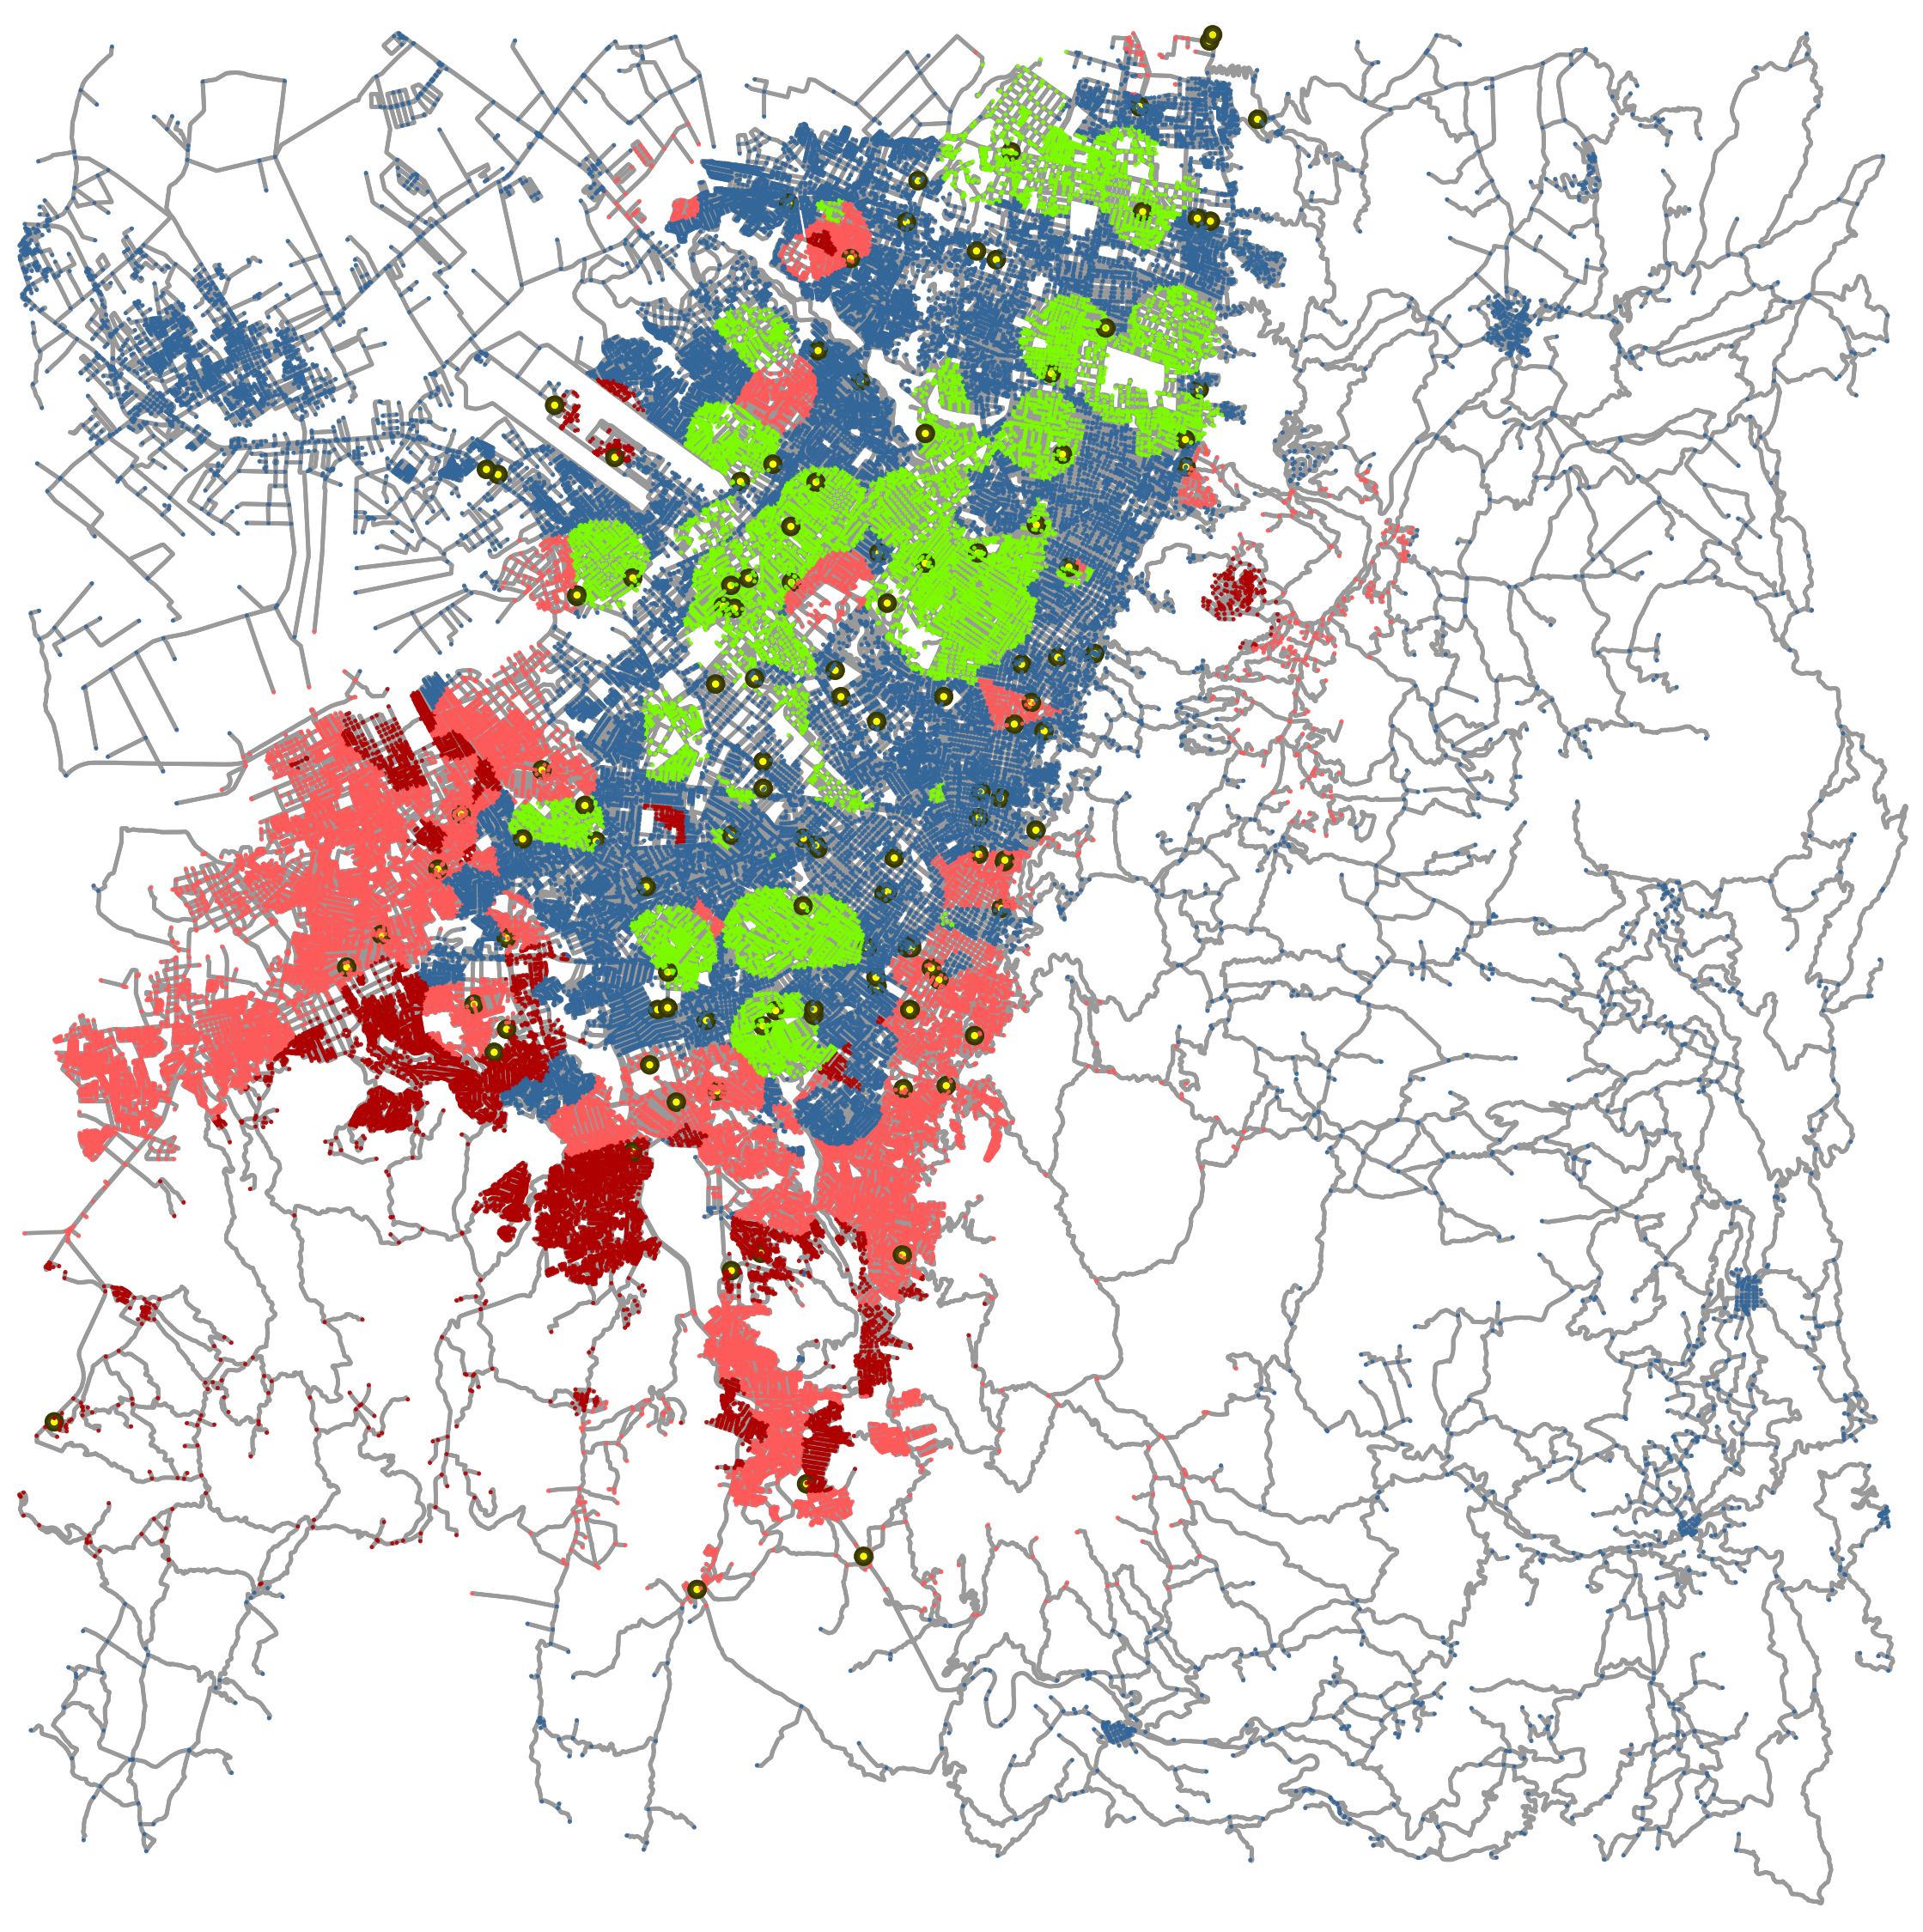
\includegraphics[width=.6\textwidth]{Images/GrafoBogotaPolicia2}
  }
  \hfill
  \subfloat[]{
  	\centering
    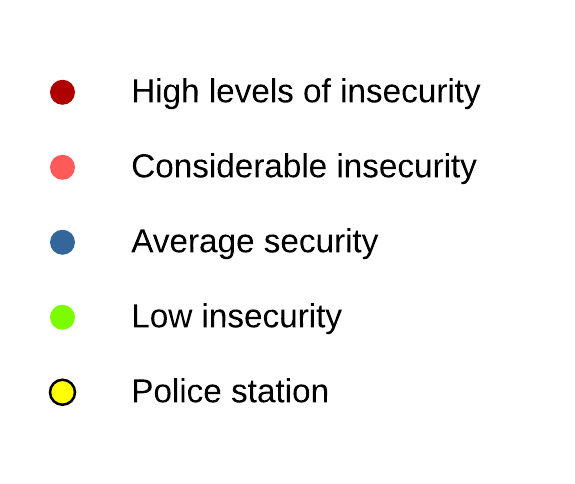
\includegraphics[width=.3\textwidth]{Images/LeyendaImagen}
  }
  \caption{Network graph representing the city of Bogotá, Colombia, as well as its surroundings, having security information represented in colors.}
  \label{fig:SafetyGraph}
\end{figure}

With respect to the police stations locations, although one can see a strong police presence in the green regions, many of the unsafe areas displayed in red have a similar amount of police stations nearby. This means that simply implementing the same number of police stations in criminal intensive neighborhoods as applied on safer zones isn't enough. The figure suggests that, before adding up more police stations, there must be an assessment of each police station's performance, including its organization, individual quality, number of active policemen, among other aspects. Naturally, there are more variables that interfere with a region's security beyond the police services. The unsafety and poverty conditions relate to how well connected the neighborhood is to central and business points of the city, as is demonstrated in the graph by the prevalence of high unsafety scores in peripheral nodes of Bogotá's street network. As such, considering the positive example of the Colombian city of Medellín in reducing crime \cite{cerda_reducing_2012}, it's safe to say that the security of Bogotá would be improved by an investment in the transport systems, mainly those that can form a stronger connection between isolated, poor regions of the city and the central, work and commercial hubs, where better social conditions, such as more jobs, education and health offers exist.


\subsection{Best Path Routing}

With every node having coordinates and scores of unsafety and traffic, the edges' weights have been updated to consider these characteristics and calculate not only a fast route, but one that is safe and that tries to avoid traffic congestions. With these new weights, the optimized path between any pair of points inside the boundaries of the current graph can be determined through the networkx package's shortest path algorithm. Afterwards, OSMnx can handle the output of networkx and plot the estimated best path over the geographically accurate graph of the city.

\begin{figure}[!h]
	\centering
	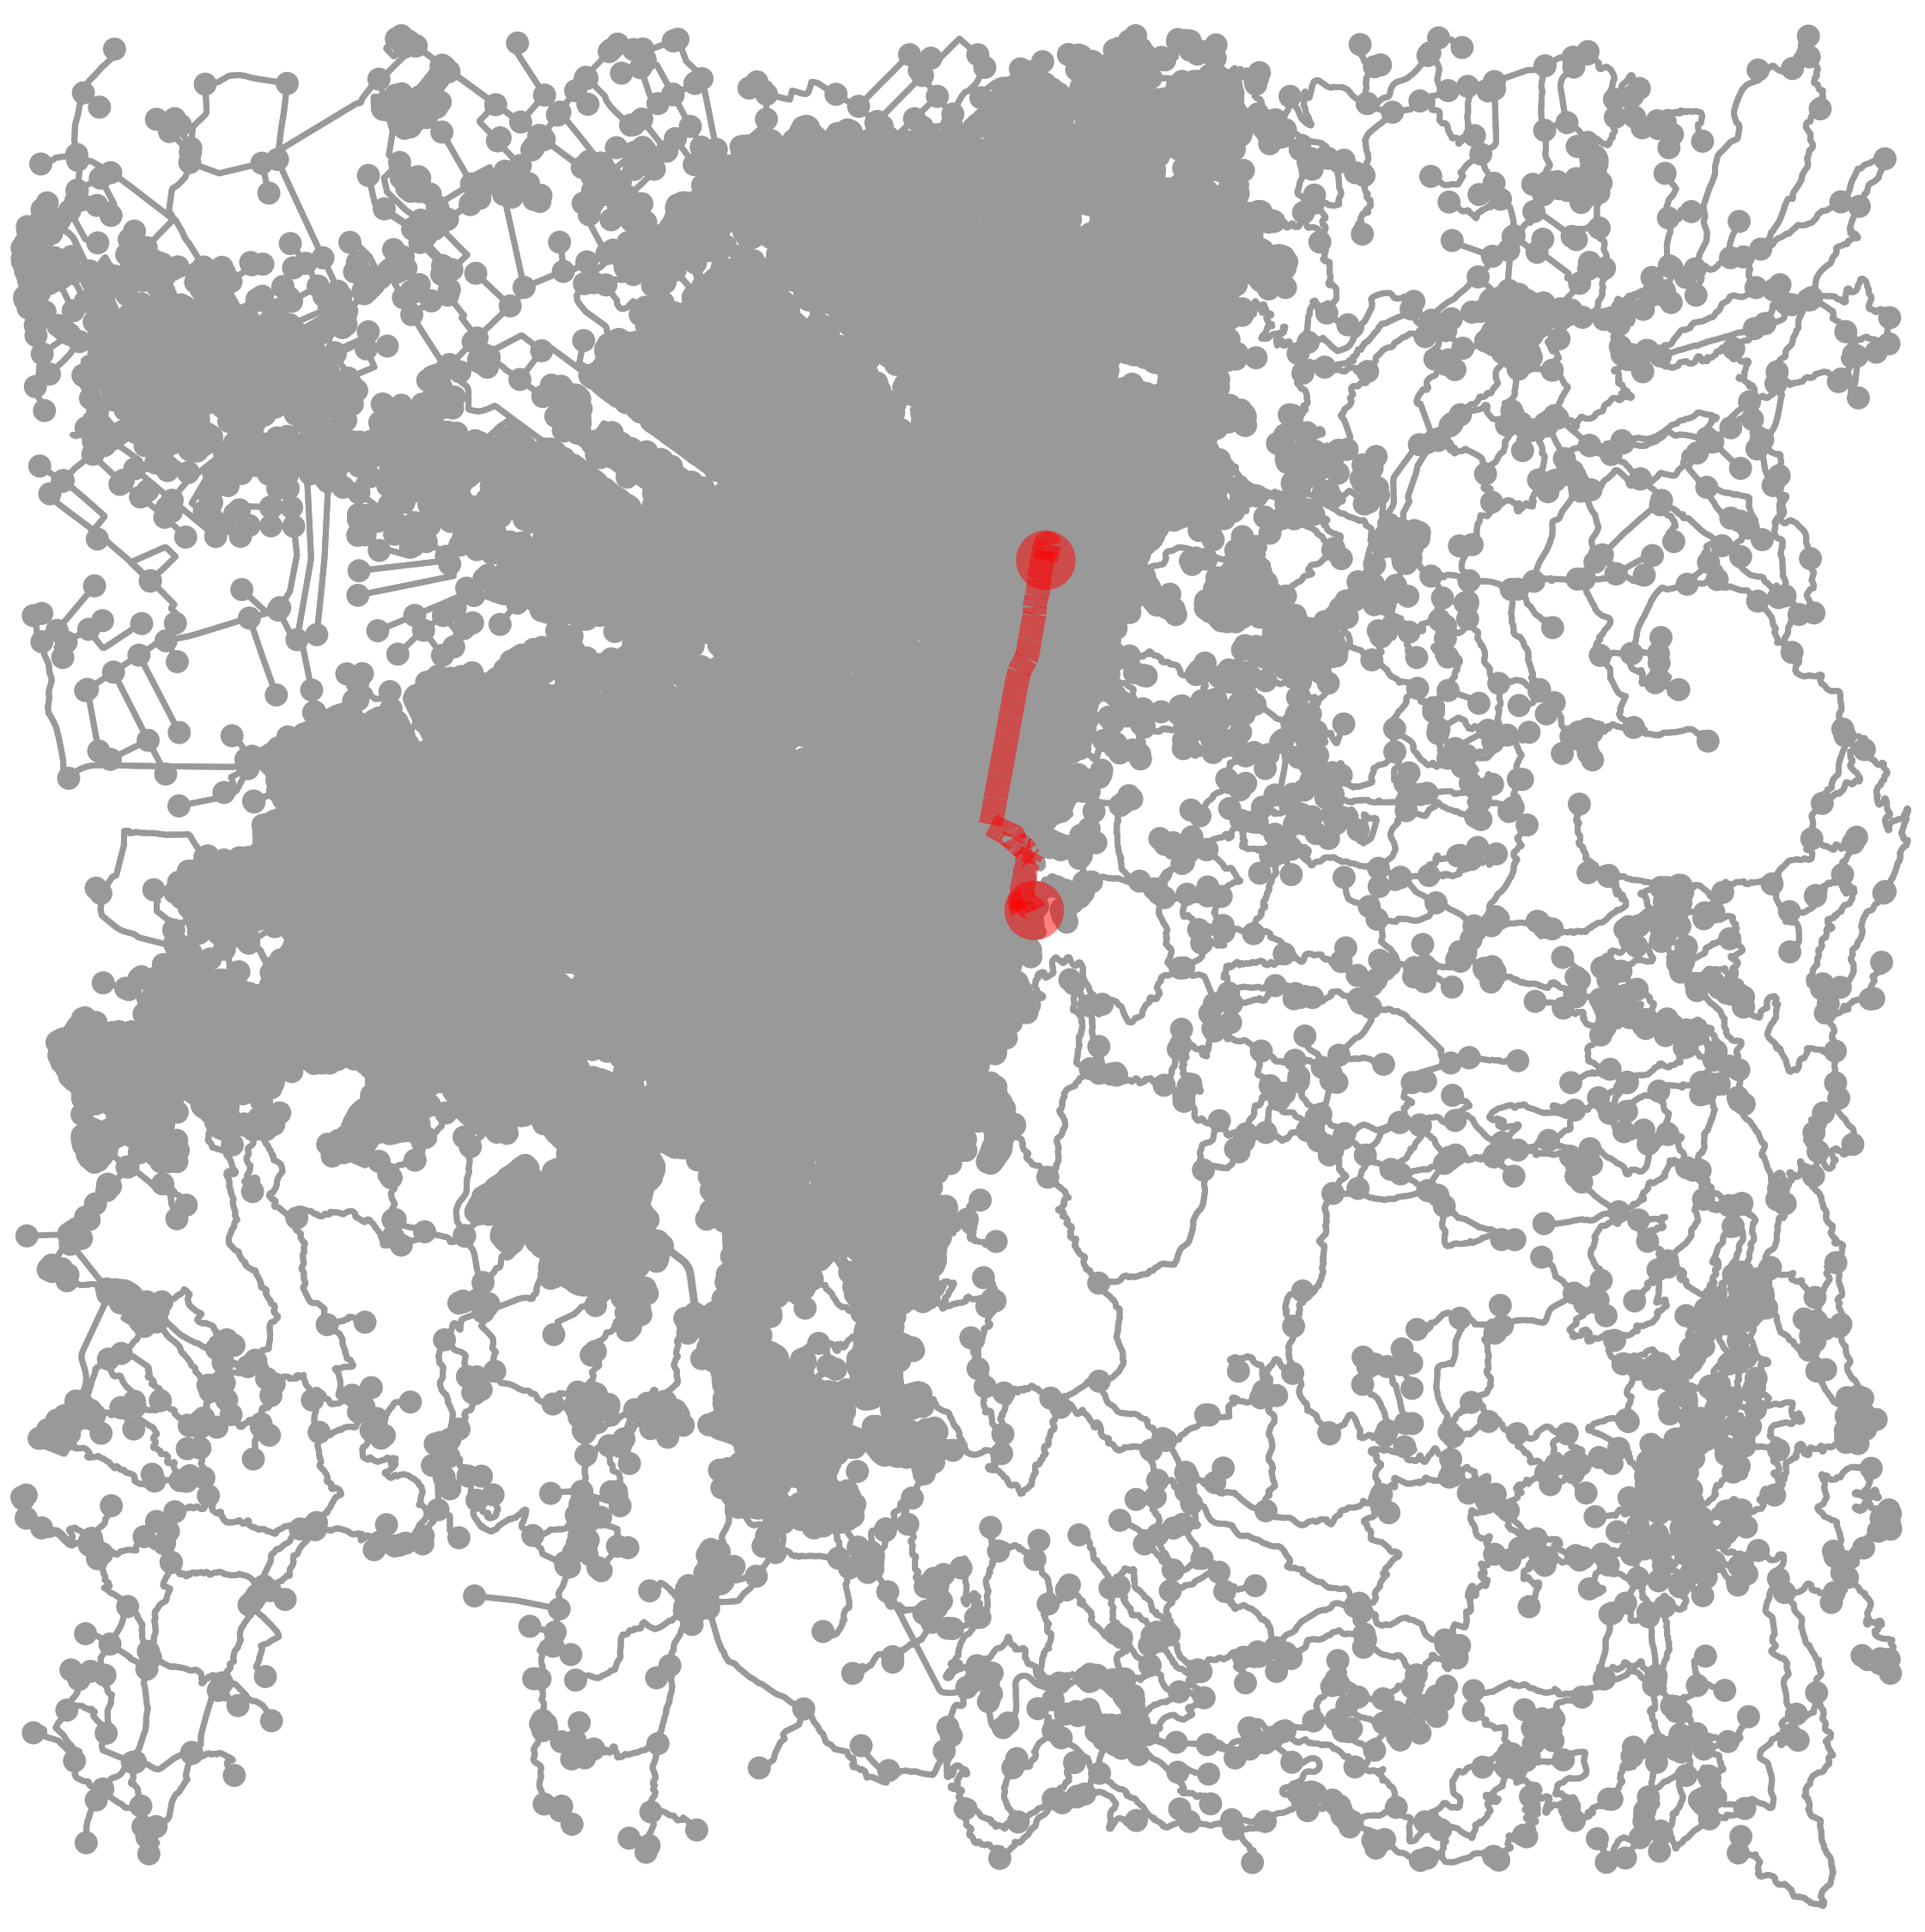
\includegraphics[width=0.5\textwidth]{Images/GrafoBogotaRutaConPesos}
	\caption{Example of an optimized least distance, safer and less traffic route between Virrey park and Monserrate, in Bogotá, Colombia.}
    \label{fig:ExampleBestRoute}
\end{figure}

As an example, figure \ref{fig:ExampleBestRoute} shows a route between the Virrey park and the local touristic attraction and religious site of Monserrate. The parameters used to get the edges' weights were $k_d = 1$, $k_s = 1$ and $k_t = \frac{1}{5000}$. These values were considered to allow a similar priority to all the three domains, being that the traffic values must be largely attenuated to be able to fairly compare with the other values, since it's around three orders of magnitude bigger than the distances and unsafety scores of the paths. Comparing with the security data from figure \ref{fig:SafetyGraph}, it's possible to see the route going in a straight line through the safer green areas, while also avoiding the dangerous boundary regions of the city, and only making a sharp turn towards to the east limit, where Monserrate is located, when it's already near the destination's latitude position.

\section{Conclusions}

In what appears to be the first urban and traffic analysis of Bogotá, Colombia, we managed to get intuitive and visual results, that can help locals get a better understanding of their city, tourists or new immigrants get to know the safety and traffic concerns, and provide tools for political institutes to take an informed decision to fight criminal activity and improve the roadway structure. By learning from the most relevant methods applied in some of the state-of-the-art urban security and traffic studies and improving upon them with novel tools implemented on a growing programming language, we consider the main achievements of this paper to be (i) getting a highly manipulable complex network representation of Bogotá, (ii) evaluating the city's regions for traffic congestion issues through population density, with a demonstration of the validity of this method while comparing with other cities, and (iii) doing a security analysis at a neighborhood level, based on real crime events and social stratum, with clear data visualization, in a city with 8 million inhabitants. While getting these results, some interesting notes were discussed, such as a proportional effect of population density and circuity on traffic congestions and the importance of effective transport connections, between the regions struggling with poverty and the main city blocks, in the reduction of crime rates and social inequality. There was also an implementation of a optimal route search, considering safety and traffic conditions alongside the distance traveled.

Considering that some of the data had manual interference, such as the parameters in calculating each node's unsafety score, as a future work it would be interesting to improve the quality of the results by finding better parameters through machine learning algorithms. There are also the possibilities of improving the security analysis by studying the criminal behavior along the course of time and hours of the day, as well as improve the traffic analysis by considering additional variables such as local circuity, connectivity, and centrality. It would also be interesting to be able to apply similar tactics to study and compare more cities across the world.


\newpage
\printbibliography

\end{document}